This chapter describes a heuristic algorithm to solve the 3D bin packing problem with vertical support.
In section \ref{sec:problem_state} we describe the concepts which will be used in the algorithm, like the definition of a state, insertions, and the feasibility of a solution.
Since the 3D-BPP is NP-Hard, an exhaustive search for a solution is not practical, so a heuristic search is conducted by combining the beam search algorithm described in \cref{sec:beamsearch} with the constructive heuristic described in \cref{sec:support_planes}.
The proposed algorithm takes in input the empty state (\ref{def:empty_state}), and outputs the best scoring state based on an ordering function defined in section \ref{ssec:scoring_states}.

\section{States}
\label{sec:problem_state}%
States or packings are partial solutions to the 3D-BPPWS. Since our heuristic is constructive by nature, the main idea of the algorithm is that by starting from a state representing an empty solution, we'll iteratively build new states that are always closer to a complete solution to the problem.
Given the formal definition of the problem (\ref{sec:milp}) we introduce a few new definitions to facilitate the algorithm's definition.
First, it is helpful to define a collection of items that still need to be assigned to a particular bin; this collection would then be used to track how many items still need to be placed.
Let us define the concept of unpacked items in relation to our MILP formulation.
\begin{definition}[Unpacked item]
    An item $i \in I$ is unpacked \textbf{iff}
    \begin{equation*}
        \sum_{b \in B} u_{ib} = 0
    \end{equation*}
\end{definition}

It is also assumed that variables identifying an item's position are independent between states (changes to their values in state $s$ won't affect state $s^\prime$).
In order to simplify the algorithm representation, rotations are handled by simply swapping the dimensions $w_i$ and $d_i$ of item $i \in I$ when needed.
A state $s$ can then be defined as follows:
\begin{itemize}
    \item $U$: the set of unpacked items,
    \item $B$: the set of used bins,
    \item $Q = (q_1, q_2,\dots, q_b)$: the set of supporting structures for each bin $b \in B$,
    \item $p$: the insertion pending on this state (described by def. \ref{def:insertion}).
\end{itemize}

Since the heuristic will open new bins when the already opened ones are full, the number of bins in each state can vary and is not fixed as a parameter to the problem like in the MILP formulation.
Thanks to the newly introduced definitions, we can trivially define a function that determines if a state is a final state.
\begin{definition}
    \label{def:state_final}
    A state $s$ is final if there are no more items to pack
    \begin{equation}
        \label{algo:state_final}%
        IsFinal(s) = \left\{\begin{aligned}
            1,\hspace{0.5cm}& s.U = \emptyset \\
            0,\hspace{0.5cm}& \text{otherwise}
        \end{aligned}
        \right.
    \end{equation}
\end{definition}

The proposed heuristic also stores additional data for each opened bin, which will then be used by the constructive heuristic described in \cref{sec:support_planes}.
This additional information is stored in the set $s.Q$ so that each bin $b \in B$ has an associated supporting structure $q_b \in s.Q$.
The collection of items placed inside a bin, for example, is one piece of data that we store in this structure.
Let us then introduce the concept of packed items inside a bin.
\begin{definition}[Packed item]
    Given a state $s$ and a bin $b \in s.B$, we say that item
    \begin{equation*}
        \begin{aligned}
            i \in I \hspace{.2cm}\text{is packed in} \hspace{.2cm}b \hspace{.2cm}& \textbf{iff} \hspace{.2cm}& u_{ib} = 1
        \end{aligned}
    \end{equation*}
\end{definition}

In addition to the set of packed items, other supporting structures are needed to facilitate checks of the problem's constraints.
Given a bin $b \in s.B$ we can then define structure $q_b$ as follows.
\begin{itemize}
    \item $J$: the set of items that are packed inside $b$,
    \item $Z$: the set of planes inside $b$ (section \ref{sec:support_planes}),
    \item $T$: the AABB Tree (section \ref{sec:problem_state:aabbtree}) representing the items inside $b$.
\end{itemize}

Both sets $q_b.J$ and $q_b.T$ contain the items packed in $b$ but adding and accessing items in $q_b.J$ has a time complexity of $O(1)$ given an implementation as hash set while maintaining $q_b.T$ usually has a time complexity of $O(log(|q_b.J|))$.

\subsection{AABB Tree}
\label{sec:problem_state:aabbtree}%

To determine the feasibility of a given state, checking for overlaps with items already placed is needed.
Since every item is a cuboid and our problem formulation only allows for $90\deg$ rotations over the z-axis, each item is contained inside a bounding box, which is axis-aligned.
An adequate structure to compute overlaps is then an Axis-Aligned Bounding Box Tree (AABB Tree) \cite{bergen1997efficient}.

AABB Trees are bounding volume hierarchies typically used for fast collision detection, and they usually offer a few operations:
\begin{itemize}
    \item $AABBInsert(i)$: which allows inserting an axis-aligned box $i$ in the tree
    \item $AABBOverlaps(i)$: which allows determining if an axis-aligned box $i$ overlaps an element in the tree
    \item $AABBClosest(i, d)$: which, given an axis-aligned box $i$ and an axis-aligned direction $d$, returns the closest element following that direction starting from the box $i$
\end{itemize}

If the tree is appropriately balanced, each operation, on average, has a time complexity of $O(log(n))$ where $n$ is the number of elements in the tree.
Maintaining an AABB Tree in the state allows us to do checks for feasibility during the construction of a solution (as detailed in \ref{ssec:scoring_insertions} ) and feasibility checks on the final states to allow for error detection.

\label{aabb:get_supporting}%
An additional opertation $AABBGetSupporting(i, \beta_s)$ was added to compute the set of supporting boxes of item $i$ given a vertical tolerance $\beta_s$.
This was possible by only checking intersections over the XY-plane similarly to the $AABBOverlaps$ implementation and filtering each item by the distance with tolerance.

\subsection{Feasibility}
\label{sec:problem_state:feasibility}%
A state $s$ is feasible if the currently packed items in each bin $b \in s.B$ aren't overlapping any other item if they are all contained inside their bin and if each item is either on the ground or satisfies at least one of the support conditions (cond. \ref{support:area_support}, cond. \ref{support:vertex_support}).
Since the proposed heuristic is constructive, it is more convenient to define the concept of feasibility relative to a change in the state.
In the heuristic, we generate new states by applying insertions starting from an initial feasible one. Let us define the concept of insertion and how an insertion is feasible.

\begin{definition}[Insertion]
    \label{def:insertion}%
    Given a state $s$, we define an insertion $p$ as a tuple $(b, I)$ where $b \in s.B$, and $I$ is a set of non-overlapping unpacked items such that they are inserted at the same $z$.
    \begin{equation*}
        \label{eq:insertion_same_z}
        I \subseteq s.U \land \exists z (z \in \mathbb{Z} \land \forall i ( i \in I \land z_i = z))
    \end{equation*}
\end{definition}
\begin{observation}
    \label{oss:state_bin_open}
    Given a state $s$ and an insertion $p = (b, \emptyset)$ where $b \notin s.B$, $p$ is an insertion that opens a new bin $b$ in $s$.
\end{observation}

\begin{definition}[Next]
    \label{def:state_next}%
    Let $p$ be an insertion over a state $s$, we define $s^\prime = Next(s, p)$ as a "copy" of state $s$ where $p$ is the pending insertion ($s^\prime.p = p$).
\end{definition}

We evaluate the changes to the score of a state based on its pending insertion. 
In this way, we don't have to update all the structures for every evaluated state. 
In addition, this property let us do fewer memory clones of states that would have been discarded either way (as seen in \cref{sec:beamsearch}). 
We can then define an algorithm that applies a pending insertion $p$ on a given state $s$ with the help of a function $OpenBin(b)$ which initializes a new structure $q_b$ with every element at its empty value.
The proposed algorithm is shown in \ref{algo:state_commit}.

\begin{algorithm}[H] \label{algo:state_commit}
    \DontPrintSemicolon
    \SetAlgoLined
    \SetKwInOut{Input}{input}
    \SetKwInOut{Output}{output}
    \Input{$s$}
    \Output{$s^\prime$}
    $(b, I) \gets s.p$\;
    $s^\prime \gets Clone(s)$\CommentSty{ //Memory clone of $s$}\;
    \If{$b \in s^\prime.B$}{
        $q_b \gets (q_i \in s^\prime.Q : i = b)$\;
        $q_b.J \gets q_b.J \cup I$\;
        $s^\prime.U \gets s^\prime.U \setminus I$\;
    }
    \Else(Open a new bin){
        $s^\prime.B \gets s^\prime.B \cup b$\;
        $s^\prime.Q \gets s^\prime.Q \cup OpenBin(b)$\;
    }
    $s^\prime.p \gets \text{none}$\;
    \Return{$s^\prime$}
    \caption{Commit}
\end{algorithm}

\paragraph*{Insertion feasibility}
An insertion $p = (b, I)$ that is pending on a given state $s$ is feasible if every inserted item $i \in p.I$ satisfies the constraint of non-overlap (\ref{cons:no_overlap}), the constraint of support (\ref{cons:every_item_is_supported}) and if it is placed within the bin.
Given an item from the set of the inserted items $i \in p.I$, and the AABB tree for bin $p.b$ in the current state $q_b.T$ as $T$.
Let $I_{\text{support}}$ be the set of items that could support item $i$ when placed in the bin, which could be saved in an appropriate structure or computed through the AABB tree as defined in \cref{aabb:get_supporting}.

Let $HasSupport(i, I_{\text{support}})$ be the function that returns true if the considered item would verify at least one of the conditions of support (cond. \ref{support:area_support} or cond. \ref{support:vertex_support}) or false otherwise.
We can define a function $IsFeasible(i, I_{\text{support}}, T)$ which returns true if the insertion of $i$ in bin $b$ for state $s$ is feasible and false otherwise. 
If every item $i \in p.I$ is feasible and every item in $I$ is not overlapping the others, then insertion $p$ is feasible.
In case some items in $p$ aren't feasible we can always define a function $RemoveInfeasibleItems(p, I_{\text{support}}, T)$ which removes every unfeasible item and returns a new insertion $p^\prime = (b, I^\prime)$ where $I^\prime = p.I \setminus \{i \in p.I : \lnot IsFeasible(i, I_{\text{support}}, T)\}$. \label{algo:remove_infeasible}

Checking if a state is feasible can then be done by iteratively applying all the insertions ordered by z and updating the proper trees, or starting from an already built tree and computing the set $I_{\text{support}}$ for each item through the tree as defined in \ref{aabb:get_supporting}.
\begin{proposition}
    \label{prop:feasible_expansion}
    A state $s^\prime$ derived by committing a feasible insertion $p$ to a feasible state $s$ is feasible.
\end{proposition}

\begin{observation}
    \label{def:empty_state}
    We can always define the empty state $s_e$ where \begin{equation*}
        \left\{ 
            \begin{aligned}
            s_e.U & = I \\
            s_e.Q & = \emptyset \\
            s_e.B & = \emptyset
            \end{aligned}
        \right.
    \end{equation*}
    and it is always feasible
\end{observation}

\subsection{State Hashing}
\label{sec:state_uniqueness}%
From a given state, it's possible to apply two different sequences of insertions and end up with two states that have all the items in the same positions.
This undesirable behavior was observed during our computational experiments.
A hashing mechanism needs to be introduced to enable checking if two states are likely the same in constant time.
In a state $s$ we can identify a packed item $i \in I$ in a given position $(x_i, y_i, z_i)$ with its given dimensions $(w_i, d_i, z_i)$ in a given bin $b \in s.B$ with a non-commutative hashing function $hash\_nc$. 
The resulting hash $hash_{ib} = hash\_nc(b, x_i, y_i, z_i, w_i, d_i, h_i)$ can identify every similar packing of an item of the same shape in that specific bin spot.
Since $hash_{ib}$ identifies one item with the shape of $i$ in the same spot as $i$, we can use a commutative function to combine every hash for every packed item in every bin to ignore the order with which items were added to the solution.
The combined hash can then be saved inside the state structure as follows. 
\begin{equation}
    s.hash = \sum\limits_{b \in s.B}{\sum\limits_{i \in q_b.J}{hash_{ib}}}
\end{equation}
In our tests, by filtering states with the proposed hash as seen in algo. \ref{algo:beamsearch}, with a simple 64-bit hashing function, this mechanism allowed us to filter out all equal states between iterations with a low amount of collisions.
Since the combining of hashes is a simple sum with modulus, the hashing of the state can also be kept updated in constant time at each iteration by simply adding the inserted hashes in the $Commit$ function (algo. \ref{algo:state_commit}).

%TODO: Do a grammar pass
\section{Beam Search}
\label{sec:beamsearch}%
%TODO: maybe add info on literature  (search about Bisiani)
Beam Search (BS) is a heuristic tree search algorithm designed for systems with limited memory where expanding every possible node is unfeasible.
The idea behind BS is to conduct an iterative truncated breadth-first search where, at each iteration, only a limited number of $k$ nodes is expanded.
After the expansion, every new node needs to be evaluated and sorted to prune the number of nodes down to the $k$ best ones. The algorithm keeps exploring until no further node can be expanded.

To perform BS one must define the node structure, an expansion function to generate new nodes from existing ones, a ranking between nodes, and a function to determine if a node is final.

A node in the tree can be represented as the state in \cref{sec:problem_state} and \cref{algo:state_final} can be used to determine if a state is final. We also know that a new state $s^\prime$ derived by $s$ by applying a feasible insertion $p$ can be computed as in \cref{def:state_next}.
This state expansion procedure, with the exception of empty insertions, will generate new states in our tree which will add a positive number of bins or packed items to the solution so, eventually, it will generate a final state.

If the starting state for the search is feasible every new state generated will be feasible and if a final state is found it will be feasible ( \cref{prop:feasible_expansion}).
We also note that starting from state $s$ the time complexity to compute feasible insertions can be lower than the complexity required to update the structures that will be used for further expansions (AABB Tree insertion and balancing, memory cloning, etc.) so we modified the standard BS algorithm to separate the expansion phase from the commit phase.
As noted in \cref{sec:state_uniqueness}, since by evaluating different insertions on different states it is possible to end up having two equal states, a filtering mechanism should be introduced.
During each iteration, it is possible to keep the hashes of the best scoring selected states in a HashSet and discard new states with the same hash.

Given a set of initial states $S^0$ and the number of best states to expand at each iteration $k$, the described BS can be represented by algorithm \ref{algo:beamsearch}.
As observed in \cref{def:empty_state}, it's possible to start the search from $S^0 = \{ s_e \}$.

\begin{algorithm}[H] \label{algo:beamsearch}
    \DontPrintSemicolon
    \SetAlgoLined
    \SetKwInOut{Input}{input}
    \SetKwInOut{Output}{output}
    \Input{$S^0, k$}
    \Output{$s_{best}$}
    $S^t \gets S^0$\;
    $S_{final} \gets \emptyset$\;
    \Repeat{$S^t \neq \emptyset $}{
        $S^{t+1} \gets Expand(S^t)$ (algo. \ref{algo:state_successor})\;
        $S_{final} \gets S_{final} \cup \{s \in S^{t+1} : IsFinal(s)\}$ (def. \ref{def:state_final})\;
        $S^{t+1} \gets S^{t+1} \setminus S_{final}$\;
        $S^{t+1} \gets Sort(S^{t+1})$ (sec. \ref{ssec:scoring_states})\;
        $S^t \gets \emptyset$\;
        $i \gets 0$\;
        $seen \gets \emptyset$\;
        \ForAll{$s \in S^{t+1}$}{
            \If{$hash^s \in seen$}{
                continue\;
            }
            $S^t \gets S^t \cup Commit(s)$ (algo. \ref{algo:state_commit})\;
            $seen \gets seen \cup \{ hash^s \}$\;
            $i \gets i+1$\;
            \If{$i > k$}{
                break\;
            }
        }
    }
    $S_{final} \gets Sort(S_{final})$\;
    \Return{best element of $S_{final}$}
    \caption{Beam search}
\end{algorithm}

\paragraph*{State Expansion}

An expansion of a state $s$ can be seen as a new set of states $S_{new}$ derived by a set of feasible insertions.
In order to determine these insertions, an underlying heuristic is used (described in \cref{sec:support_planes}).

The main idea in this phase of the algorithm is to find feasible insertions in all the bins at the lowest possible height for items that still need to be packed.
To reduce the number of possible expansions to evaluate we limit the search to insertions of items with unique shapes.
With a similar concept to the one used in \cref{sec:state_uniqueness}, an hash for each item's dimensions can be computed on the fly or pre-computed as a problem's parameter.
Given each item's hash we can then group items that have the same shape.
The evaluation of new insertions can then be done with two different approaches:
\begin{itemize}
    \label{def:placement_modes}%
    \item \textbf{PS}: where we evaluate only the possible insertion of a single item per item type, which would generate insertions of at most 1 item,
    \item \textbf{PM}: where we evaluate the biggest possible insertion of a group of items of the same shape, which would generate insertions of at most the size of the group of items with the same shape.
\end{itemize}
Creating insertions of groups of similar items is usually used in Pallet Loading Problems (as for ex. \cite{elhedhli2019three}) to create better bases of support for upper layers.
With a similar intuition, the idea of placing groups of items of the same shape is to facilitate the creation of uniform planes (not necessarily layers) to use for further insertions.

Given a set of items $I$ and a tolerance $\beta_s$ we can introduce an algorithm to group them by their shape and produce a set $G$ of tuples $(h, I^\prime)$ where $h$ is the hash summurizing the shape of the group and $I^\prime$ is the set of items grouped as in algo. \ref{algo:group_by_hash}.
Once items are grouped by shape the best insertion for each class of items can be computed for each open bin. If no insertion is possible in any bin, then the only viable insertion is the bin opening insertion (\cref{oss:state_bin_open}).
The described procedure is detailed in algo. \ref{algo:state_successor}, which can be modified with minor changes to limit the number of items to consider when in PS mode.

\begin{algorithm}[H] \label{algo:state_successor}
    \DontPrintSemicolon
    \SetAlgoLined
    \SetKwInOut{Input}{input}
    \SetKwInOut{Output}{output}
    \Input{$S$}
    \Output{$S_{new}$}
    \ForAll{$s \in S$}{
        $S_{new} \leftarrow \emptyset$\;
        $I_{family} \leftarrow GroupByFamily(s.Unpacked)$\;
        %$minPlacement \leftarrow \{(b, 0) | \forall b \in s.Bins \}$\;
        $placed \leftarrow false$\;
        \ForAll{$(family, I) \in I_{family}$}{
            \ForAll{$bin \in s.Bins$}{
                $placement \leftarrow SPBestInsertion(s, bin, I)$ (Algorithm \ref{algo:sp_bestinsertion})\;
                \If{$placement \neq \emptyset$}{
                    $placed \leftarrow true$\;
                    %$minPlacement(bin) \leftarrow min(minPlacement(bin), placement.z)$\;
                    %TODO: abuso di notazione
                    $S_{new} \leftarrow S_{new} \cup Next(s, placement)$\;
                }
            }
        }
        \If{$placed = false$}{
            $S_{new} \leftarrow S_{new} \cup OpenNewBin(s)$\;
        }
        %TODO: Filter?
    }
    \Return{$S_{new}$}
    \caption{Expand}
\end{algorithm}
\begin{algorithm}[ht] \label{algo:group_by_hash}
    \DontPrintSemicolon
    \SetAlgoLined
    \SetKwInOut{Input}{input}
    \SetKwInOut{Output}{output}
    \Input{$I$}
    \Output{$G$}
    $G \gets \emptyset$\;
    \ForAll{$i \in I$}{
        $generate \gets \text{true}$\;
        \ForAll{$(h, I^\prime) \in G$}{
            \If{$h = hash(w_i, d_i, h_i)$}{
                $generate \gets \text{false}$\;
                $I^\prime \gets I^\prime \cup i$\;
                break\;
            }
        }
        \If{$generate = \text{true}$}{
            $G \gets G \cup (hash(w_i, d_i, h_i), \{ i \})$\;
        }
    }
    \Return{$G$}
    \caption{Group By Hash}
\end{algorithm}


\subsection{Scoring States}
\label{ssec:scoring_states}%
In order to sort states, a scoring function needs to be defined over them.
Since the scoring of the states is what will influence the final solution the most, parameters that are directly related to minimizing the objective function are selected.

In the proposed solution to handle multiple objective functions, lexicographic ordering is used.
\begin{definition}
    \label{def:lexicographic_ordering}
    Let $f_1(s), f_2(s), f_i(s), \dots, f_n(s)$ be objective functions ordered by precedence based on index $i \in \mathbb{Z}$, then 
    \begin{equation*}
        s < s^\prime \hspace{.2cm} \textbf{iff} \hspace{.2cm} \exists j \in \mathbb{Z} : \left\{
            \begin{aligned}
                f_j(s) < f_j(s^\prime) & \\
                f_k(s) = f_k(s^\prime) &,\hspace{.5cm} \forall k \in \mathbb{Z} : 0 \le k < j 
            \end{aligned}
        \right.
    \end{equation*}
\end{definition}

Scoring metrics for each state $s$ that we want to evaluate can then be computed in the $Next$ algorithm by considering the contents of the pending insertions and updating each parameter differentially.

The defined ordering utilized is the following:
\begin{itemize}
    \item $f_1(s) = -|s.B|$: we prefer states that opened fewer bins.
    \item $f_2(s) = \text{avgvol}(s)$: we prefer states that have packed more average volume between bins.
    \item $f_3(s) = \text{avgcageratio}(s)$: we prefer states that have better average cage ratio (\cref{eq:cage_ratio}) between bins.
\end{itemize}

\section{Support Planes}
\label{sec:support_planes}%
Support Planes (SP) is a constructive heuristic based on an underlying 2D-BPP heuristic which is used to generate feasible insertions inside a bin starting from a set of items to pack.
Since insertions must be feasible, SP maintains an internal structure to facilitate feasibility checks.
The idea at the base of SP is to build a solution to the 3D-BPP by filling 2D planes called \textit{support planes}.

Each support plane is characterized by the tuple $(z, I_{support}, I_{upper})$ where
\begin{itemize}
    \item $z$: is the height of the plane,
    \item $I_{support}$: the set of the items that can offer support to items placed on the plane,
    \item $I_{upper}$: the set of items that will be obstacles to potential new items placed on the plane.
\end{itemize}

Every item placed in the bin can either generate a new support plane or be part of the supporting items of other planes. 
Items placed above a particular plane, such that $z_i + h_i > z$, are considered obstacles and are added to the $I_{upper}$ set.
When evaluating a new possible insertion, given a set of items to place $I$, SP selects the first feasible insertion starting from the lowest plane by using a modified version of Extreme Point in two dimensions (introduced in \cite{crainic2008extreme}).
Once no more insertions can be made on the lowest available support plane, it's removed from the set of planes.
Since insertions always happen in the lowest possible planes, the set of obstacles of those planes is composed of items that have only their top face above the $z$ of the evaluated plane, such that $z_i \le z < z_i + h_i$.

The Extreme Point (EP) heuristic evaluates the placement of rectangles in a plane based on a set of reference points with a best-fit approach. 
Each rectangle placement generates a new set of reference points which are usually introduced based on the projection of its corner points along the orthogonal axis of the plane.
The corner points of an added rectangle $r$ placed in $(x_r, y_r)$ of dimensions $(w_r, d_r)$ are the top left corner $(x_r, y_r + d_r)$ and the bottom right corner $(x_r + w_r, y_r)$.
In our version of the algorithm, the corner points of each item are introduced without projecting them to increase the likelihood of evaluating placements that verify the support constraint.
Placements follow a first-fit approach where the algorithm selects the first point closest to the origin where a rectangle can fit with or without rotations.
In order to facilitate the evaluation of reference points with support, we also generate a reference point in the bottom left corner of each item that belongs to the set of supporting items $I_{support}$.
When a reference point is used for a placement, it is then removed from the pool of reference points.
Before evaluating placements, the item to place are ordered based on their area.
New planes have the origin of space $(0,0)$ as an available reference point.

Since reference points are usually ordered based on the euclidean distance from the bottom left corner of the plane and the corner points are usually generated and projected towards the origin of each axis, the placements over one plane are usually biased towards the bottom left corner.
To address the problem, we evaluate four instances of EP where each has a different coordinate change applied to every item that moves the plane's origin to each corner of the bin.
This addition is based on similar approaches from the literature where it is usually used to more uniformly fill the space (ex. \citeauthor{GAJDA2022102559}) and was verified to yield better cage ratio results in our internal testing.
%TODO: Check the above

The EP procedure is called for each item to pack on a given plane. 
In order to produce a valid insertion, every item in the insertion shouldn't overlap each other (as stated in \cref{def:insertion}).
Since the AABB tree for a given state is shared by each evaluation of a possible insertion, it can't be modified to account for temporary placements of items.
This means that we need to keep a temporary AABB tree updated composed of the items that are part of the current insertion $T^\prime$.
We can then define a function that uses the temporary tree and the feasibility function defined in \cref{sec:problem_state:feasibility} to ensure that we are producing a feasible insertion as \cref{eq:ep_can_pack}.
\begin{equation}
    \label{eq:ep_can_pack}
    EPCanPack(i, I_{support}, T, T^\prime) = IsFeasible(i, I_{support}, T) \land \lnot AABBOverlaps(i, T^\prime)
\end{equation}
A graphical representation of a support plane is shown in \cref{fig:support_planes} with the reference points available. In \cref{fig:ep_coordinate_changes} the state of two extreme point instances for the bottom left and top left coordinate changes are shown.
When a bin is opened the only support plane available is the one on the ground. 
In the figure different coordinate changes are marked with different colors.

\begin{figure}[hp]
    \centering
    \scalebox{0.9}{%
    

\tikzset{every picture/.style={line width=0.75pt}} %set default line width to 0.75pt        

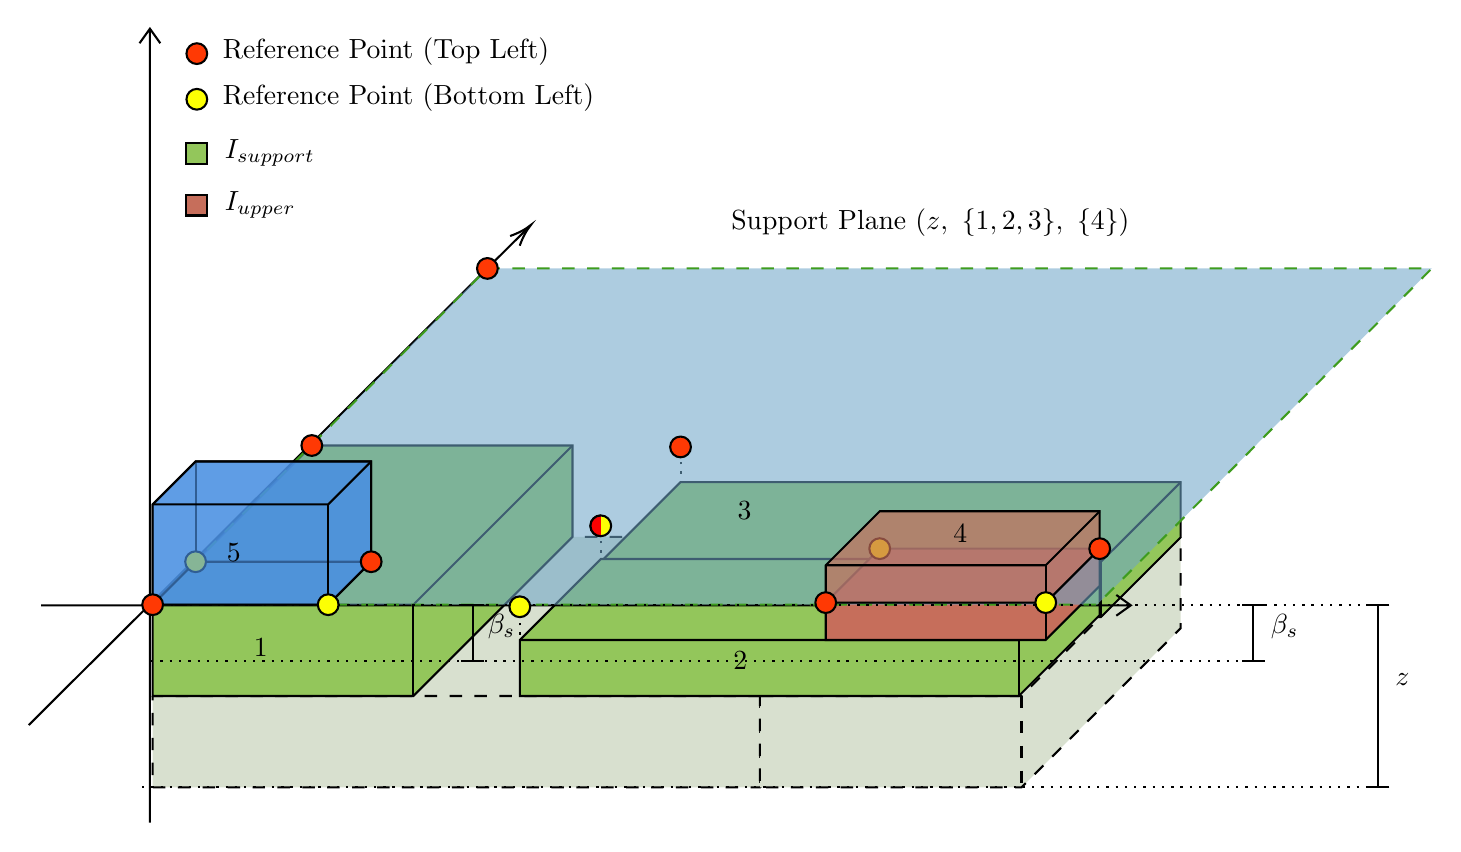
\begin{tikzpicture}[x=0.75pt,y=0.75pt,yscale=-1,xscale=1]
%uncomment if require: \path (0,412); %set diagram left start at 0, and has height of 412

%Shape: Cube [id:dp7106500856615827] 
\draw  [fill={rgb, 255:red, 216; green, 224; blue, 207 }  ,fill opacity=1 ][dash pattern={on 4.5pt off 4.5pt}] (69.7,334.5) -- (146.4,257.81) -- (439,257.81) -- (439,301.81) -- (362.31,378.5) -- (69.7,378.5) -- cycle ; \draw  [dash pattern={on 4.5pt off 4.5pt}] (439,257.81) -- (362.31,334.5) -- (69.7,334.5) ; \draw  [dash pattern={on 4.5pt off 4.5pt}] (362.31,334.5) -- (362.31,378.5) ;
%Straight Lines [id:da8316956251676535] 
\draw  [dash pattern={on 0.84pt off 2.51pt}]  (285.62,269.89) -- (285.62,252.5) ;
%Straight Lines [id:da38384433092333237] 
\draw  [dash pattern={on 0.84pt off 2.51pt}]  (324.05,231.89) -- (324.05,214.5) ;
%Shape: Cube [id:dp47709739603214574] 
\draw  [fill={rgb, 255:red, 216; green, 224; blue, 207 }  ,fill opacity=1 ][dash pattern={on 4.5pt off 4.5pt}] (362.31,334.5) -- (439,257.81) -- (565,257.81) -- (565,301.81) -- (488.31,378.5) -- (362.31,378.5) -- cycle ; \draw  [dash pattern={on 4.5pt off 4.5pt}] (565,257.81) -- (488.31,334.5) -- (362.31,334.5) ; \draw  [dash pattern={on 4.5pt off 4.5pt}] (488.31,334.5) -- (488.31,378.5) ;
%Shape: Cube [id:dp7977002200403227] 
\draw  [fill={rgb, 255:red, 147; green, 198; blue, 91 }  ,fill opacity=1 ] (69.7,290.5) -- (146.4,213.81) -- (272,213.81) -- (272,257.81) -- (195.31,334.5) -- (69.7,334.5) -- cycle ; \draw   (272,213.81) -- (195.31,290.5) -- (69.7,290.5) ; \draw   (195.31,290.5) -- (195.31,334.5) ;
%Shape: Cube [id:dp7121611670665484] 
\draw  [fill={rgb, 255:red, 147; green, 198; blue, 91 }  ,fill opacity=1 ] (285.62,269.89) -- (324.05,231.46) -- (565,231.46) -- (565,258.06) -- (526.56,296.5) -- (285.62,296.5) -- cycle ; \draw   (565,231.46) -- (526.56,269.89) -- (285.62,269.89) ; \draw   (526.56,269.89) -- (526.56,296.5) ;
%Shape: Cube [id:dp604763542929154] 
\draw  [fill={rgb, 255:red, 147; green, 198; blue, 91 }  ,fill opacity=1 ] (246.62,307.5) -- (285.62,268.5) -- (526,268.5) -- (526,295.5) -- (487,334.5) -- (246.62,334.5) -- cycle ; \draw   (526,268.5) -- (487,307.5) -- (246.62,307.5) ; \draw   (487,307.5) -- (487,334.5) ;
%Shape: Axis 2D [id:dp786981943451631] 
\draw  (16,290.81) -- (541,290.81)(68.4,13) -- (68.4,395.5) (534,285.81) -- (541,290.81) -- (534,295.81) (63.4,20) -- (68.4,13) -- (73.4,20)  ;
%Straight Lines [id:da31524103851047525] 
\draw    (10,348.5) -- (250.58,108.91) ;
\draw [shift={(252,107.5)}, rotate = 135.12] [color={rgb, 255:red, 0; green, 0; blue, 0 }  ][line width=0.75]    (10.93,-3.29) .. controls (6.95,-1.4) and (3.31,-0.3) .. (0,0) .. controls (3.31,0.3) and (6.95,1.4) .. (10.93,3.29)   ;
%Shape: Cube [id:dp6424617162036526] 
\draw  [fill={rgb, 255:red, 198; green, 110; blue, 91 }  ,fill opacity=1 ] (394,289.5) -- (420,263.5) -- (526,263.5) -- (526,281.5) -- (500,307.5) -- (394,307.5) -- cycle ; \draw   (526,263.5) -- (500,289.5) -- (394,289.5) ; \draw   (500,289.5) -- (500,307.5) ;
%Shape: Parallelogram [id:dp3639839698249763] 
\draw  [color={rgb, 255:red, 62; green, 156; blue, 30 }  ,draw opacity=1 ][fill={rgb, 255:red, 110; green, 165; blue, 200 }  ,fill opacity=0.57 ][dash pattern={on 4.5pt off 4.5pt}] (231,128.5) -- (686,128.5) -- (524.7,290.5) -- (69.7,290.5) -- cycle ;
%Straight Lines [id:da11997650250706615] 
\draw    (659.96,290.5) -- (659.96,378.5) ;
\draw [shift={(659.96,378.5)}, rotate = 270] [color={rgb, 255:red, 0; green, 0; blue, 0 }  ][line width=0.75]    (0,5.59) -- (0,-5.59)   ;
\draw [shift={(659.96,290.5)}, rotate = 270] [color={rgb, 255:red, 0; green, 0; blue, 0 }  ][line width=0.75]    (0,5.59) -- (0,-5.59)   ;
%Straight Lines [id:da7479086158615895] 
\draw  [dash pattern={on 0.84pt off 2.51pt}]  (69.7,290.5) -- (665,290.5) ;
%Straight Lines [id:da00936893511639092] 
\draw  [dash pattern={on 0.84pt off 2.51pt}]  (64.66,378.5) -- (659.96,378.5) ;
%Straight Lines [id:da2603505755036556] 
\draw  [dash pattern={on 0.84pt off 2.51pt}]  (69,317.5) -- (600,317.5) ;
%Straight Lines [id:da21695403696781168] 
\draw    (600,290.5) -- (600,317.5) ;
\draw [shift={(600,317.5)}, rotate = 270] [color={rgb, 255:red, 0; green, 0; blue, 0 }  ][line width=0.75]    (0,5.59) -- (0,-5.59)   ;
\draw [shift={(600,290.5)}, rotate = 270] [color={rgb, 255:red, 0; green, 0; blue, 0 }  ][line width=0.75]    (0,5.59) -- (0,-5.59)   ;
%Straight Lines [id:da17628222853988207] 
\draw    (224,290.5) -- (224,317.5) ;
\draw [shift={(224,317.5)}, rotate = 270] [color={rgb, 255:red, 0; green, 0; blue, 0 }  ][line width=0.75]    (0,5.59) -- (0,-5.59)   ;
\draw [shift={(224,290.5)}, rotate = 270] [color={rgb, 255:red, 0; green, 0; blue, 0 }  ][line width=0.75]    (0,5.59) -- (0,-5.59)   ;
%Shape: Cube [id:dp458320338188952] 
\draw  [fill={rgb, 255:red, 74; green, 144; blue, 226 }  ,fill opacity=0.66 ] (175,269.8) -- (154.3,290.5) -- (69.7,290.5) -- (69.7,242.2) -- (90.4,221.5) -- (175,221.5) -- cycle ; \draw   (69.7,290.5) -- (90.4,269.8) -- (175,269.8) ; \draw   (90.4,269.8) -- (90.4,221.5) ;
%Shape: Circle [id:dp9728798663710179] 
\draw  [fill={rgb, 255:red, 252; green, 255; blue, 4 }  ,fill opacity=1 ] (86,47) .. controls (86,44.24) and (88.24,42) .. (91,42) .. controls (93.76,42) and (96,44.24) .. (96,47) .. controls (96,49.76) and (93.76,52) .. (91,52) .. controls (88.24,52) and (86,49.76) .. (86,47) -- cycle ;
%Shape: Circle [id:dp41733873180988235] 
\draw  [fill={rgb, 255:red, 252; green, 255; blue, 4 }  ,fill opacity=1 ] (85.4,269.8) .. controls (85.4,267.04) and (87.64,264.8) .. (90.4,264.8) .. controls (93.17,264.8) and (95.4,267.04) .. (95.4,269.8) .. controls (95.4,272.56) and (93.17,274.8) .. (90.4,274.8) .. controls (87.64,274.8) and (85.4,272.56) .. (85.4,269.8) -- cycle ;
%Shape: Cube [id:dp9609158816144449] 
\draw  [fill={rgb, 255:red, 74; green, 144; blue, 226 }  ,fill opacity=0.66 ] (69.7,242.2) -- (90.4,221.5) -- (175,221.5) -- (175,269.8) -- (154.3,290.5) -- (69.7,290.5) -- cycle ; \draw   (175,221.5) -- (154.3,242.2) -- (69.7,242.2) ; \draw   (154.3,242.2) -- (154.3,290.5) ;
%Shape: Circle [id:dp7069570068237806] 
\draw  [fill={rgb, 255:red, 252; green, 255; blue, 4 }  ,fill opacity=1 ] (149.3,290.5) .. controls (149.3,287.74) and (151.54,285.5) .. (154.3,285.5) .. controls (157.06,285.5) and (159.3,287.74) .. (159.3,290.5) .. controls (159.3,293.26) and (157.06,295.5) .. (154.3,295.5) .. controls (151.54,295.5) and (149.3,293.26) .. (149.3,290.5) -- cycle ;
%Shape: Circle [id:dp07493756825553233] 
\draw  [fill={rgb, 255:red, 252; green, 255; blue, 4 }  ,fill opacity=1 ] (241.62,291.5) .. controls (241.62,288.74) and (243.86,286.5) .. (246.62,286.5) .. controls (249.38,286.5) and (251.62,288.74) .. (251.62,291.5) .. controls (251.62,294.26) and (249.38,296.5) .. (246.62,296.5) .. controls (243.86,296.5) and (241.62,294.26) .. (241.62,291.5) -- cycle ;
%Shape: Circle [id:dp9652867077591403] 
\draw  [fill={rgb, 255:red, 252; green, 255; blue, 4 }  ,fill opacity=1 ] (280.62,252.5) .. controls (280.62,249.74) and (282.86,247.5) .. (285.62,247.5) .. controls (288.38,247.5) and (290.62,249.74) .. (290.62,252.5) .. controls (290.62,255.26) and (288.38,257.5) .. (285.62,257.5) .. controls (282.86,257.5) and (280.62,255.26) .. (280.62,252.5) -- cycle ;
%Straight Lines [id:da7143423337159592] 
\draw  [dash pattern={on 0.84pt off 2.51pt}]  (246.62,313.89) -- (246.62,296.5) ;
%Shape: Rectangle [id:dp672375593139905] 
\draw  [fill={rgb, 255:red, 147; green, 198; blue, 91 }  ,fill opacity=1 ] (86,68) -- (96,68) -- (96,78) -- (86,78) -- cycle ;
%Shape: Rectangle [id:dp16133242915286994] 
\draw  [fill={rgb, 255:red, 198; green, 110; blue, 91 }  ,fill opacity=1 ] (86,93) -- (96,93) -- (96,103) -- (86,103) -- cycle ;
%Shape: Circle [id:dp7335317400317659] 
\draw  [fill={rgb, 255:red, 255; green, 57; blue, 4 }  ,fill opacity=1 ] (86,25) .. controls (86,22.24) and (88.24,20) .. (91,20) .. controls (93.76,20) and (96,22.24) .. (96,25) .. controls (96,27.76) and (93.76,30) .. (91,30) .. controls (88.24,30) and (86,27.76) .. (86,25) -- cycle ;
%Shape: Circle [id:dp4790782266696906] 
\draw  [fill={rgb, 255:red, 255; green, 57; blue, 4 }  ,fill opacity=1 ] (319.05,214.5) .. controls (319.05,211.74) and (321.29,209.5) .. (324.05,209.5) .. controls (326.82,209.5) and (329.05,211.74) .. (329.05,214.5) .. controls (329.05,217.26) and (326.82,219.5) .. (324.05,219.5) .. controls (321.29,219.5) and (319.05,217.26) .. (319.05,214.5) -- cycle ;
%Shape: Circle [id:dp3675058769915285] 
\draw  [fill={rgb, 255:red, 255; green, 57; blue, 4 }  ,fill opacity=1 ] (141.4,213.81) .. controls (141.4,211.05) and (143.63,208.81) .. (146.4,208.81) .. controls (149.16,208.81) and (151.4,211.05) .. (151.4,213.81) .. controls (151.4,216.57) and (149.16,218.81) .. (146.4,218.81) .. controls (143.63,218.81) and (141.4,216.57) .. (141.4,213.81) -- cycle ;
%Shape: Circle [id:dp6836568323907531] 
\draw  [fill={rgb, 255:red, 255; green, 57; blue, 4 }  ,fill opacity=1 ] (170,269.8) .. controls (170,267.04) and (172.24,264.8) .. (175,264.8) .. controls (177.76,264.8) and (180,267.04) .. (180,269.8) .. controls (180,272.56) and (177.76,274.8) .. (175,274.8) .. controls (172.24,274.8) and (170,272.56) .. (170,269.8) -- cycle ;
%Shape: Circle [id:dp9319287698621804] 
\draw  [fill={rgb, 255:red, 255; green, 57; blue, 4 }  ,fill opacity=1 ] (64.7,290.5) .. controls (64.7,287.74) and (66.94,285.5) .. (69.7,285.5) .. controls (72.47,285.5) and (74.7,287.74) .. (74.7,290.5) .. controls (74.7,293.26) and (72.47,295.5) .. (69.7,295.5) .. controls (66.94,295.5) and (64.7,293.26) .. (64.7,290.5) -- cycle ;
%Shape: Arc [id:dp7222867806291037] 
\draw  [draw opacity=0][fill={rgb, 255:red, 251; green, 1; blue, 1 }  ,fill opacity=1 ] (285.62,257.5) .. controls (285.62,257.5) and (285.62,257.5) .. (285.62,257.5) .. controls (285.62,257.5) and (285.62,257.5) .. (285.62,257.5) .. controls (282.86,257.5) and (280.62,255.26) .. (280.62,252.5) .. controls (280.62,249.74) and (282.86,247.5) .. (285.62,247.5) -- (285.62,252.5) -- cycle ; \draw   (285.62,257.5) .. controls (285.62,257.5) and (285.62,257.5) .. (285.62,257.5) .. controls (285.62,257.5) and (285.62,257.5) .. (285.62,257.5) .. controls (282.86,257.5) and (280.62,255.26) .. (280.62,252.5) .. controls (280.62,249.74) and (282.86,247.5) .. (285.62,247.5) ;  
%Shape: Circle [id:dp7431470261343242] 
\draw  [fill={rgb, 255:red, 252; green, 255; blue, 4 }  ,fill opacity=1 ] (415,263.5) .. controls (415,260.74) and (417.24,258.5) .. (420,258.5) .. controls (422.76,258.5) and (425,260.74) .. (425,263.5) .. controls (425,266.26) and (422.76,268.5) .. (420,268.5) .. controls (417.24,268.5) and (415,266.26) .. (415,263.5) -- cycle ;
%Shape: Cube [id:dp46874066075395426] 
\draw  [fill={rgb, 255:red, 198; green, 110; blue, 91 }  ,fill opacity=0.69 ] (394,271.5) -- (420,245.5) -- (526,245.5) -- (526,263.5) -- (500,289.5) -- (394,289.5) -- cycle ; \draw   (526,245.5) -- (500,271.5) -- (394,271.5) ; \draw   (500,271.5) -- (500,289.5) ;
%Shape: Circle [id:dp4546060900911436] 
\draw  [fill={rgb, 255:red, 252; green, 255; blue, 4 }  ,fill opacity=1 ] (495,289.5) .. controls (495,286.74) and (497.24,284.5) .. (500,284.5) .. controls (502.76,284.5) and (505,286.74) .. (505,289.5) .. controls (505,292.26) and (502.76,294.5) .. (500,294.5) .. controls (497.24,294.5) and (495,292.26) .. (495,289.5) -- cycle ;
%Shape: Circle [id:dp1099531157368071] 
\draw  [fill={rgb, 255:red, 255; green, 57; blue, 4 }  ,fill opacity=1 ] (521,263.5) .. controls (521,260.74) and (523.24,258.5) .. (526,258.5) .. controls (528.76,258.5) and (531,260.74) .. (531,263.5) .. controls (531,266.26) and (528.76,268.5) .. (526,268.5) .. controls (523.24,268.5) and (521,266.26) .. (521,263.5) -- cycle ;
%Shape: Circle [id:dp6477599340697807] 
\draw  [fill={rgb, 255:red, 255; green, 57; blue, 4 }  ,fill opacity=1 ] (389,289.5) .. controls (389,286.74) and (391.24,284.5) .. (394,284.5) .. controls (396.76,284.5) and (399,286.74) .. (399,289.5) .. controls (399,292.26) and (396.76,294.5) .. (394,294.5) .. controls (391.24,294.5) and (389,292.26) .. (389,289.5) -- cycle ;
%Shape: Circle [id:dp38665130344221843] 
\draw  [fill={rgb, 255:red, 255; green, 57; blue, 4 }  ,fill opacity=1 ] (226,128.5) .. controls (226,125.74) and (228.24,123.5) .. (231,123.5) .. controls (233.76,123.5) and (236,125.74) .. (236,128.5) .. controls (236,131.26) and (233.76,133.5) .. (231,133.5) .. controls (228.24,133.5) and (226,131.26) .. (226,128.5) -- cycle ;

% Text Node
\draw (667,322.4) node [anchor=north west][inner sep=0.75pt]    {$z$};
% Text Node
\draw (347,98) node [anchor=north west][inner sep=0.75pt]   [align=left] {Support Plane $\displaystyle ( z,\ \{1,2,3\} ,\ \{4\})$};
% Text Node
\draw (104,259.4) node [anchor=north west][inner sep=0.75pt]    {$5$};
% Text Node
\draw (117,305.4) node [anchor=north west][inner sep=0.75pt]    {$1$};
% Text Node
\draw (348,311.4) node [anchor=north west][inner sep=0.75pt]    {$2$};
% Text Node
\draw (350,239.4) node [anchor=north west][inner sep=0.75pt]    {$3$};
% Text Node
\draw (454,250.4) node [anchor=north west][inner sep=0.75pt]    {$4$};
% Text Node
\draw (607,293.4) node [anchor=north west][inner sep=0.75pt]    {$\beta _{s}$};
% Text Node
\draw (229.67,293.4) node [anchor=north west][inner sep=0.75pt]    {$\beta _{s}$};
% Text Node
\draw (102,38) node [anchor=north west][inner sep=0.75pt]   [align=left] {Reference Point (Bottom Left)};
% Text Node
\draw (103,65) node [anchor=north west][inner sep=0.75pt]   [align=left] {$\displaystyle I_{support}$};
% Text Node
\draw (103,90) node [anchor=north west][inner sep=0.75pt]   [align=left] {$\displaystyle I_{upper}$};
% Text Node
\draw (102,16) node [anchor=north west][inner sep=0.75pt]   [align=left] {Reference Point (Top Left)};


\end{tikzpicture}

    }
    \caption{Representation of a generic support plane with a placed item}
    \label{fig:support_planes}
\end{figure}

\begin{figure}[hp]
    \centering
    %\scalebox{0.75}{%
    

\tikzset{every picture/.style={line width=0.75pt}} %set default line width to 0.75pt        

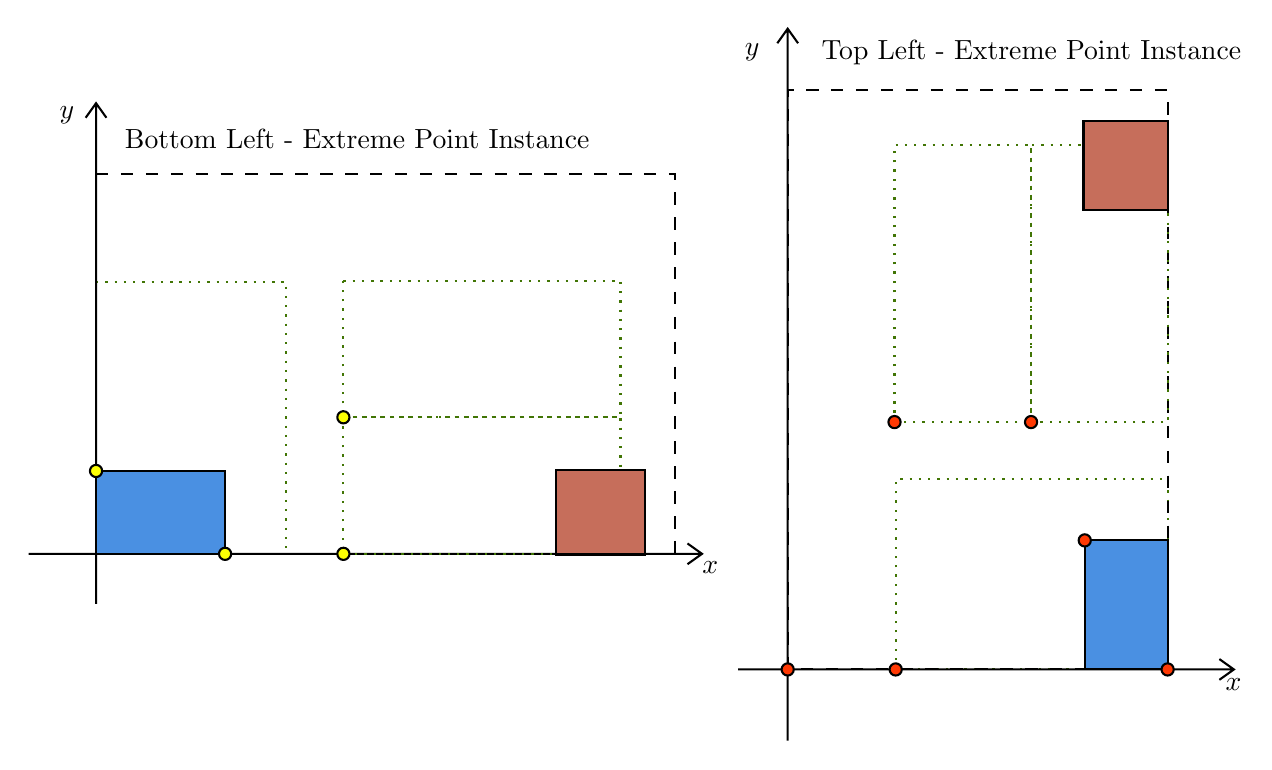
\begin{tikzpicture}[x=0.75pt,y=0.75pt,yscale=-1,xscale=1]
%uncomment if require: \path (0,380); %set diagram left start at 0, and has height of 380

%Shape: Rectangle [id:dp676391404304541] 
\draw  [color={rgb, 255:red, 65; green, 117; blue, 5 }  ,draw opacity=1 ][dash pattern={on 0.84pt off 2.51pt}] (65.44,151.69) -- (157,151.69) -- (157,282.71) -- (65.44,282.71) -- cycle ;
%Shape: Rectangle [id:dp26001178837889305] 
\draw  [color={rgb, 255:red, 65; green, 117; blue, 5 }  ,draw opacity=1 ][dash pattern={on 0.84pt off 2.51pt}] (450.7,338.41) -- (450.7,246.85) -- (581.72,246.85) -- (581.72,338.41) -- cycle ;
%Shape: Rectangle [id:dp532870934725963] 
\draw  [dash pattern={on 4.5pt off 4.5pt}] (65.44,99.66) -- (344.58,99.66) -- (344.58,282.71) -- (65.44,282.71) -- cycle ;
%Shape: Axis 2D [id:dp545947560183275] 
\draw  (33,282.71) -- (357.39,282.71)(65.44,65.6) -- (65.44,306.84) (350.39,277.71) -- (357.39,282.71) -- (350.39,287.71) (60.44,72.6) -- (65.44,65.6) -- (70.44,72.6)  ;
%Shape: Rectangle [id:dp13640021794487145] 
\draw  [fill={rgb, 255:red, 74; green, 144; blue, 226 }  ,fill opacity=1 ] (65.44,242.78) -- (127.61,242.78) -- (127.61,282.71) -- (65.44,282.71) -- cycle ;
%Shape: Ellipse [id:dp4997787088203596] 
\draw  [fill={rgb, 255:red, 252; green, 255; blue, 4 }  ,fill opacity=1 ] (62.5,242.78) .. controls (62.5,241.16) and (63.82,239.84) .. (65.44,239.84) .. controls (67.06,239.84) and (68.38,241.16) .. (68.38,242.78) .. controls (68.38,244.4) and (67.06,245.72) .. (65.44,245.72) .. controls (63.82,245.72) and (62.5,244.4) .. (62.5,242.78) -- cycle ;
%Shape: Ellipse [id:dp9368091558454169] 
\draw  [fill={rgb, 255:red, 252; green, 255; blue, 4 }  ,fill opacity=1 ] (124.67,282.71) .. controls (124.67,281.09) and (125.99,279.77) .. (127.61,279.77) .. controls (129.24,279.77) and (130.55,281.09) .. (130.55,282.71) .. controls (130.55,284.34) and (129.24,285.65) .. (127.61,285.65) .. controls (125.99,285.65) and (124.67,284.34) .. (124.67,282.71) -- cycle ;
%Shape: Rectangle [id:dp10130767347226488] 
\draw  [color={rgb, 255:red, 65; green, 117; blue, 5 }  ,draw opacity=1 ][dash pattern={on 0.84pt off 2.51pt}] (184.62,216.92) -- (318.13,216.92) -- (318.13,282.71) -- (184.62,282.71) -- cycle ;
%Shape: Rectangle [id:dp8859988076373574] 
\draw  [color={rgb, 255:red, 65; green, 117; blue, 5 }  ,draw opacity=1 ][dash pattern={on 0.84pt off 2.51pt}] (184.62,151.14) -- (318.13,151.14) -- (318.13,216.92) -- (184.62,216.92) -- cycle ;
%Shape: Rectangle [id:dp5346376956315015] 
\draw  [fill={rgb, 255:red, 198; green, 110; blue, 91 }  ,fill opacity=1 ] (286.87,242.19) -- (329.77,242.19) -- (329.77,283.04) -- (286.87,283.04) -- cycle ;
%Shape: Ellipse [id:dp5380867242688693] 
\draw  [fill={rgb, 255:red, 252; green, 255; blue, 4 }  ,fill opacity=1 ] (181.68,282.71) .. controls (181.68,281.09) and (182.99,279.77) .. (184.62,279.77) .. controls (186.24,279.77) and (187.55,281.09) .. (187.55,282.71) .. controls (187.55,284.34) and (186.24,285.65) .. (184.62,285.65) .. controls (182.99,285.65) and (181.68,284.34) .. (181.68,282.71) -- cycle ;
%Shape: Circle [id:dp32824759445274065] 
\draw  [fill={rgb, 255:red, 252; green, 255; blue, 4 }  ,fill opacity=1 ] (181.68,216.92) .. controls (181.68,215.3) and (182.99,213.99) .. (184.62,213.99) .. controls (186.24,213.99) and (187.55,215.3) .. (187.55,216.92) .. controls (187.55,218.55) and (186.24,219.86) .. (184.62,219.86) .. controls (182.99,219.86) and (181.68,218.55) .. (181.68,216.92) -- cycle ;
%Shape: Rectangle [id:dp013806976369067359] 
\draw  [dash pattern={on 4.5pt off 4.5pt}] (398.67,338.41) -- (398.67,59.27) -- (581.72,59.27) -- (581.72,338.41) -- cycle ;
%Shape: Axis 2D [id:dp26544149420697416] 
\draw  (374.78,338.41) -- (613.65,338.41)(398.67,29.71) -- (398.67,372.71) (606.65,333.41) -- (613.65,338.41) -- (606.65,343.41) (393.67,36.71) -- (398.67,29.71) -- (403.67,36.71)  ;
%Shape: Rectangle [id:dp4452985784509189] 
\draw  [fill={rgb, 255:red, 74; green, 144; blue, 226 }  ,fill opacity=1 ] (541.79,338.41) -- (541.79,276.23) -- (581.72,276.23) -- (581.72,338.41) -- cycle ;
%Shape: Rectangle [id:dp24524128214266327] 
\draw  [color={rgb, 255:red, 65; green, 117; blue, 5 }  ,draw opacity=1 ][dash pattern={on 0.84pt off 2.51pt}] (515.93,219.23) -- (515.93,85.71) -- (581.72,85.71) -- (581.72,219.23) -- cycle ;
%Shape: Rectangle [id:dp5234703657507643] 
\draw  [color={rgb, 255:red, 65; green, 117; blue, 5 }  ,draw opacity=1 ][dash pattern={on 0.84pt off 2.51pt}] (450.14,219.23) -- (450.14,85.71) -- (515.93,85.71) -- (515.93,219.23) -- cycle ;
%Shape: Rectangle [id:dp9419058705222738] 
\draw  [fill={rgb, 255:red, 198; green, 110; blue, 91 }  ,fill opacity=1 ] (541.2,116.98) -- (541.2,74.08) -- (582.04,74.08) -- (582.04,116.98) -- cycle ;
%Shape: Ellipse [id:dp3331578572136539] 
\draw  [fill={rgb, 255:red, 255; green, 57; blue, 4 }  ,fill opacity=1 ] (450.14,222.17) .. controls (448.52,222.17) and (447.21,220.85) .. (447.21,219.23) .. controls (447.21,217.61) and (448.52,216.29) .. (450.14,216.29) .. controls (451.77,216.29) and (453.08,217.61) .. (453.08,219.23) .. controls (453.08,220.85) and (451.77,222.17) .. (450.14,222.17) -- cycle ;
%Shape: Ellipse [id:dp23570925769851603] 
\draw  [fill={rgb, 255:red, 255; green, 57; blue, 4 }  ,fill opacity=1 ] (515.93,222.17) .. controls (514.31,222.17) and (512.99,220.85) .. (512.99,219.23) .. controls (512.99,217.61) and (514.31,216.29) .. (515.93,216.29) .. controls (517.56,216.29) and (518.87,217.61) .. (518.87,219.23) .. controls (518.87,220.85) and (517.56,222.17) .. (515.93,222.17) -- cycle ;
%Shape: Ellipse [id:dp6429169005498813] 
\draw  [fill={rgb, 255:red, 255; green, 57; blue, 4 }  ,fill opacity=1 ] (398.67,341.35) .. controls (397.04,341.35) and (395.73,340.03) .. (395.73,338.41) .. controls (395.73,336.78) and (397.04,335.47) .. (398.67,335.47) .. controls (400.29,335.47) and (401.6,336.78) .. (401.6,338.41) .. controls (401.6,340.03) and (400.29,341.35) .. (398.67,341.35) -- cycle ;
%Shape: Ellipse [id:dp5636473664839672] 
\draw  [fill={rgb, 255:red, 255; green, 57; blue, 4 }  ,fill opacity=1 ] (450.7,341.35) .. controls (449.08,341.35) and (447.76,340.03) .. (447.76,338.41) .. controls (447.76,336.78) and (449.08,335.47) .. (450.7,335.47) .. controls (452.33,335.47) and (453.64,336.78) .. (453.64,338.41) .. controls (453.64,340.03) and (452.33,341.35) .. (450.7,341.35) -- cycle ;
%Shape: Ellipse [id:dp310194773919646] 
\draw  [fill={rgb, 255:red, 255; green, 57; blue, 4 }  ,fill opacity=1 ] (581.72,341.35) .. controls (580.1,341.35) and (578.78,340.03) .. (578.78,338.41) .. controls (578.78,336.78) and (580.1,335.47) .. (581.72,335.47) .. controls (583.34,335.47) and (584.66,336.78) .. (584.66,338.41) .. controls (584.66,340.03) and (583.34,341.35) .. (581.72,341.35) -- cycle ;
%Shape: Ellipse [id:dp4413085834987862] 
\draw  [fill={rgb, 255:red, 255; green, 57; blue, 4 }  ,fill opacity=1 ] (541.79,279.17) .. controls (540.17,279.17) and (538.85,277.86) .. (538.85,276.23) .. controls (538.85,274.61) and (540.17,273.29) .. (541.79,273.29) .. controls (543.41,273.29) and (544.73,274.61) .. (544.73,276.23) .. controls (544.73,277.86) and (543.41,279.17) .. (541.79,279.17) -- cycle ;

% Text Node
\draw (46.39,65.64) node [anchor=north west][inner sep=0.75pt]    {$y$};
% Text Node
\draw (356.09,284.84) node [anchor=north west][inner sep=0.75pt]    {$x$};
% Text Node
\draw (77.86,76.79) node [anchor=north west][inner sep=0.75pt]   [align=left] {Bottom Left - Extreme Point Instance};
% Text Node
\draw (376.52,35.3) node [anchor=north west][inner sep=0.75pt]    {$y$};
% Text Node
\draw (608.21,341.49) node [anchor=north west][inner sep=0.75pt]    {$x$};
% Text Node
\draw (413.49,33.94) node [anchor=north west][inner sep=0.75pt]   [align=left] {Top Left - Extreme Point Instance};


\end{tikzpicture}

    %}
    \caption{Extreme Point instances for some coordinate changes of \cref{fig:support_planes}}
    \label{fig:ep_coordinate_changes}
\end{figure}
%TODO: Proporre la versione ibrida maxrect/extreme points?

Given \cref{eq:ep_can_pack} to check if a considered placement would lead to a feasible insertion, the set of items to pack $I$, the AABB tree of the currently packed items $T$ and the set of currently available support planes $Z$.
The heuristic that will output the new best possible feasible insertion for the given set of items or an empty object can be summarized in alg. \ref{algo:sp_bestinsertion}. 

\begin{algorithm}[hp]
    \DontPrintSemicolon
    \SetAlgoLined
    \SetKwInOut{Input}{input}
    \SetKwInOut{Output}{output}
    \Input{$Z, I, T$}
    \Output{$p$}
    \ForAll{$(z, I_{support}, I_{upper}) \in Z$}{
        $P \gets \emptyset$\;
        \ForAll{possible coordinate changes}{
            $p \leftarrow (z, \emptyset)$\;
            $T^\prime \gets \text{empty AABB tree}$\;
            \CommentSty{//Initialize reference points}\;
            $refPoints \gets (0,0)$\;
            \ForAll{$i \in I_{support}$}{
                $refPoints \gets refPoints \cup \{(x_i, y_i)\}$\;
            }
            \ForAll{$i \in I_{upper}$}{
                $refPoints \gets refPoints \cup \{(x_i + w_i, y_i), (x_i, y_i + d_i)\}$\;
            }
            $sort(refPoints)$ \CommentSty{// Based on euclidean distance from $(0,0)$}\;

            \CommentSty{//Create a feasible insertion for the given items}\;
            \ForAll{$i \in I$}{
                \CommentSty{//Evaluate first possible placement}\;
                \ForAll{$(x,y) \in refPoints$}{
                    $(x_i, y_i, z_i) \gets (x, y, z)$\;
                    \If{$EPCanPlace(i, T, T^\prime)$}{
                        $EPInsertRect(p, i, T^\prime, refPoints)$ \CommentSty{// alg. \ref{algo:ep_insert_rect}}\;
                        break\;
                    }
                    $(w_i, d_i) \gets (d_i, w_i)$ \CommentSty{//Try rotating $i$}\;
                    \If{$EPCanPlace(i, T, T^\prime)$}{
                        $EPInsertRect(p, i, T^\prime, refPoints)$ \CommentSty{// alg. \ref{algo:ep_insert_rect}}\;
                        break\;
                    }
                    $(w_i, d_i) \gets (d_i, w_i)$ \CommentSty{//Restore original $i$ rotation}\;
                }
            }
            \If{$p \neq (z, \emptyset)$}{
                $P \gets P \cup \{ p \}$\;
            }
        }
        $sort(P)$ \CommentSty{//Sorted as in \cref{ssec:scoring_insertions}}\;
        \If{$P \neq \emptyset$}{
            \Return{first element of $P$}
        }
    }
    \Return{none}
    \caption{SP Best Insertion \label{algo:sp_bestinsertion}}
\end{algorithm}
\begin{algorithm}[htb] 
    \DontPrintSemicolon
    \SetAlgoLined
    \SetKwInOut{Input}{input}
    \SetKwInOut{Output}{output}
    \Input{ $p, i, T, refPoints$}
    $refPoints \gets refPoints \setminus \{ (x_i, y_i) \}$\;
    $refPoints \gets refPoints \cup \{(x_i + w_i, y_i), (x_i, y_i + d_i)\}$\;
    $sort(refPoints)$ \CommentSty{// Based on euclidean distance from $(0,0)$}\;
    $p.I \gets p.I \cup \{ i \}$\;
    $AABBInsert(i, T^\prime)$ \CommentSty{//\cref{sec:problem_state:aabbtree}}\;
    \Return
    \caption{EP Insert Rect \label{algo:ep_insert_rect}}
\end{algorithm}

\paragraph*{Commit Extension}
We now describe an extension to $Commit$ (algo. \ref{algo:state_commit}) to update the structures needed by SP.

When a plane is filled, new insertions become less likely to be feasible. 
To avoid evaluating planes where no insertion is possible a mechanism to prune dead planes can be introduced.

Since best insertions for a bin are always evaluated by considering lower planes first, if all the insertions in $Expand$ (algo. \ref{algo:state_successor}) happened over a $z_{min}$ then we can safely remove the opened planes with $z < z_{min}$ for that bin.
Let us introduce a $z_{min}$ variable carried over in $q_b$ for each bin, which is updated during the $Expand$ phase with the minimum $z$ of all the insertions on bin $b$.
Once the best states are computed and $Commit$ is called we can then use its value to prune planes in each $q_b$.
Other operations are also necessary in the $Commit$ algorithm to allow SP to update its data structures accordingly to the insertion.

Given a state $s$ and an insertion $p$ where each packed item $i \in p.I$ in bin $b$ has $z_i$ within tolerance of $z$ and the minimum height for the considered bin $q_b.z_{min}$.
The algorithm which updates the structures for a given bin $b$ is represented by algorithm \ref{algo:sp_commit}.
This new algorithm can be used as the last step of the $Commit$ algorithm for each $b \in s^\prime.B$.

\begin{algorithm}[H] \label{algo:sp_commit}
    \DontPrintSemicolon
    \SetAlgoLined
    \SetKwInOut{Input}{input}
    \SetKwInOut{Output}{output}
    \SetSideCommentRight
    \Input{$s_b, I, z, z_{min}, t$}
    \Output{$s^\prime_b$}
    \CommentSty{//Filter bad planes}\;
    $P^\prime \leftarrow planes \setminus \{ \forall S_z \in planes : z \le z_{min} \}$\;
    \CommentSty{//Apply insertion}\;
    $B \leftarrow placed \cup I$\;
    $U \leftarrow unpacked \setminus I$\;
    $T \leftarrow aabb$\;
    \ForAll{$i \in I$}{
        $T \leftarrow InsertAABB(i, T)$ \CommentSty{//If balanced $O(log(n))$}\; %TODO: specify balanced
        $generate \leftarrow true$\;
        % O(|P'|)
        \ForAll{$S^\prime_z \in P^\prime$}{ %TODO: specify balanced
            \CommentSty{//Based on the distance from the top of the item}\;
            $dz \leftarrow S^\prime_z.z - i.z_{max}$\;
            \If{$0 \le dz \le t$}{
                $generate \leftarrow false$\;
                $S^\prime_z.I_{support} \leftarrow S^\prime_z.I_{support} \cup i$\;
            } \ElseIf{$dz < 0$}{
                $S^\prime_z.I_{upper} \leftarrow S^\prime_z.I_{upper} \cup i$\;
            }
        }

        \If{$generate$}{
            $P^\prime \leftarrow P^\prime \cup (i.z_{max}, \{i\}, \emptyset)$\;
        }
    }
    \Return{$Update(s_b, P^\prime, B, U, T)$}
    \caption{SP Apply and Filter}
\end{algorithm}

\subsection{Scoring Insertions}
\label{ssec:scoring_insertions}%
Similarly to the scoring of states (\cref{ssec:scoring_states}), an ordering function is also needed to evaluate different insertions for the same set of items.
Given the lexicographic ordering formulation in \cref{def:lexicographic_ordering} a few new statistics can be calculated and stored inside an insertion to help in the evaluation.
The parameters used to sort an insertion $p$ are then the following:
\begin{itemize}
    \item $f_1(p) = -|p.I|$: maximize number of items inserted (of the same shape),
    \item $f_2(p) = -\sum\limits_{i \in p.I}{(w_i d_i + w_i d_i h_i)}$: maximize the sum of the area and volume of each packed item,
    \item $f_3(p) = \max\limits_{i \in p.I}(z_i + h_i)$: minimize the maximum height of the inserted items,
    \item $f_4(p) = \text{sum of the supported area of items in $p.I$}$: minimize the support area available to the inserted items,
    \item $f_5(p) = $
\end{itemize}
%TODO: more in depth